
\subsection{Überblick über den Umrichter-Prüfstand}
\label{subsec:uberblick-uber-den-umrichter-prufstand}

In diesem Abschnitt wird der Umrichter-Teststand, von dem die zu verarbeitenden Datensätze stammen beschrieben,
da dies für das generelle Verständnis der einzulesenden Datensatzstruktur unerlässlich ist.
Die genaue Bezeichnung des Teststandes „USTB DWT Test Bench (XCT0006-1)“ im weiteren als Test-Bench oder Teststand benannt.
Diese Art Test-Bench wird im allgemein für die End-of-Line Prüfung von unterschiedlichen Umrichtern nach ihrer Herstellung genutzt,
um die Produktqualität und -funktionalität sicherzustellen.\cite*{Main_Manuel_USTB2018}

In dem hier vorliegenden Fall wird der Teststand verwendet, um die aus dem Feld kommenden Umrichter auf ihre weitere Nutzungstauglichkeit zu testen.
Die weitere Nutzungstauglichkeit wird ermittelt, indem die Messwerte mit Mittelwerten, die von mehreren fabrikneuen Umrichtern stammenden verglichen werden.
Diese Messwerte müssen sich in einen vorher definierten Toleranzbereich befinden, um weiter in Feld verwenden zu werden.

Die Umrichter werden in der gegebenen Fachliteratur zur Test-Bench als \ac{DUTs} bezeichnet.
Diese Bezeichnung kommt auch in den Berichten aud dem Teststand vor, daher hat der Autor diese Abkürzung übernommen.
%------------------------------------------------------------------------------------------------------
\subsubsection{Aufbau des Teststandes}
%------------------------------------------------------------------------------------------------------
Die Test-Bench besteht aus mehreren Komponenten, die sich im Testraum in unterschiedlichen Schaltschränken befinden.
Der Teststand besteht aus folgenden Hauptkomponenten:

\begin{itemize}

\item Das Netzteil wandelt die 400V Netzspannung in eine isolierte Gleichspannung für den Zwischenkreis um.
Das Netzteil leifert maximal 80kW mit 1200VDC oder 800VDC, welche Werte verwendet werden kann vor Teststart bestimmt werden.
In Abbildung \ref{fig:1. Aufbau des Teststandes} mit PSU bezeichnet, für „Power Supply Unit“.
\item Das Elektronik-Rack, auf dem Mess- und Control-Komponenten befestigt sind.
Hier befinden sich auch der (XCS2100) System-Controller der das ganze System mit dem PC, auf dem die Test-Bench Software läuft, via Ethernet verbindet.
In Abbildung \ref{fig:1. Aufbau des Teststandes} mit ER bezeichnet, für „Electronic Rack“.
\item Der Testmatrix-Schrank, in dem die Sammelschienen für den Stromanschluss und den Schützen sitzen.
In Abbildung \ref{fig:1. Aufbau des Teststandes} mit TM bezeichnet, für „Test Matrix cabine“.
\item Der Schrank mit dem Kühlungssystem, da die Umrichter während des Betriebes Wasser oder Luft gekühlt werden müssen.
In Abbildung \ref{fig:1. Aufbau des Teststandes} mit „Cool1“ bezeichnet.
\item Dem Carrier, auf dem Umrichter befestigt werden.
Dieser wird speziell für bestimmte Umrichter konstruiert.
In Abbildung \ref{fig:1. Aufbau des Teststandes} mit Carrier1 bezeichnet.

\end{itemize}

Neben dem Hauptkomponenten befinden sich außerhalb des Sicherheitsbereiches, der während des Betriebes nicht betreten werden darf,
ein PC mit einer Software zum Steuern der Testeinrichtung, sowie eine Betriebsanzeige und ein Notaus. \cite*{Main_Manuel_USTB2018}

\begin{figure}[h]
    \centering
    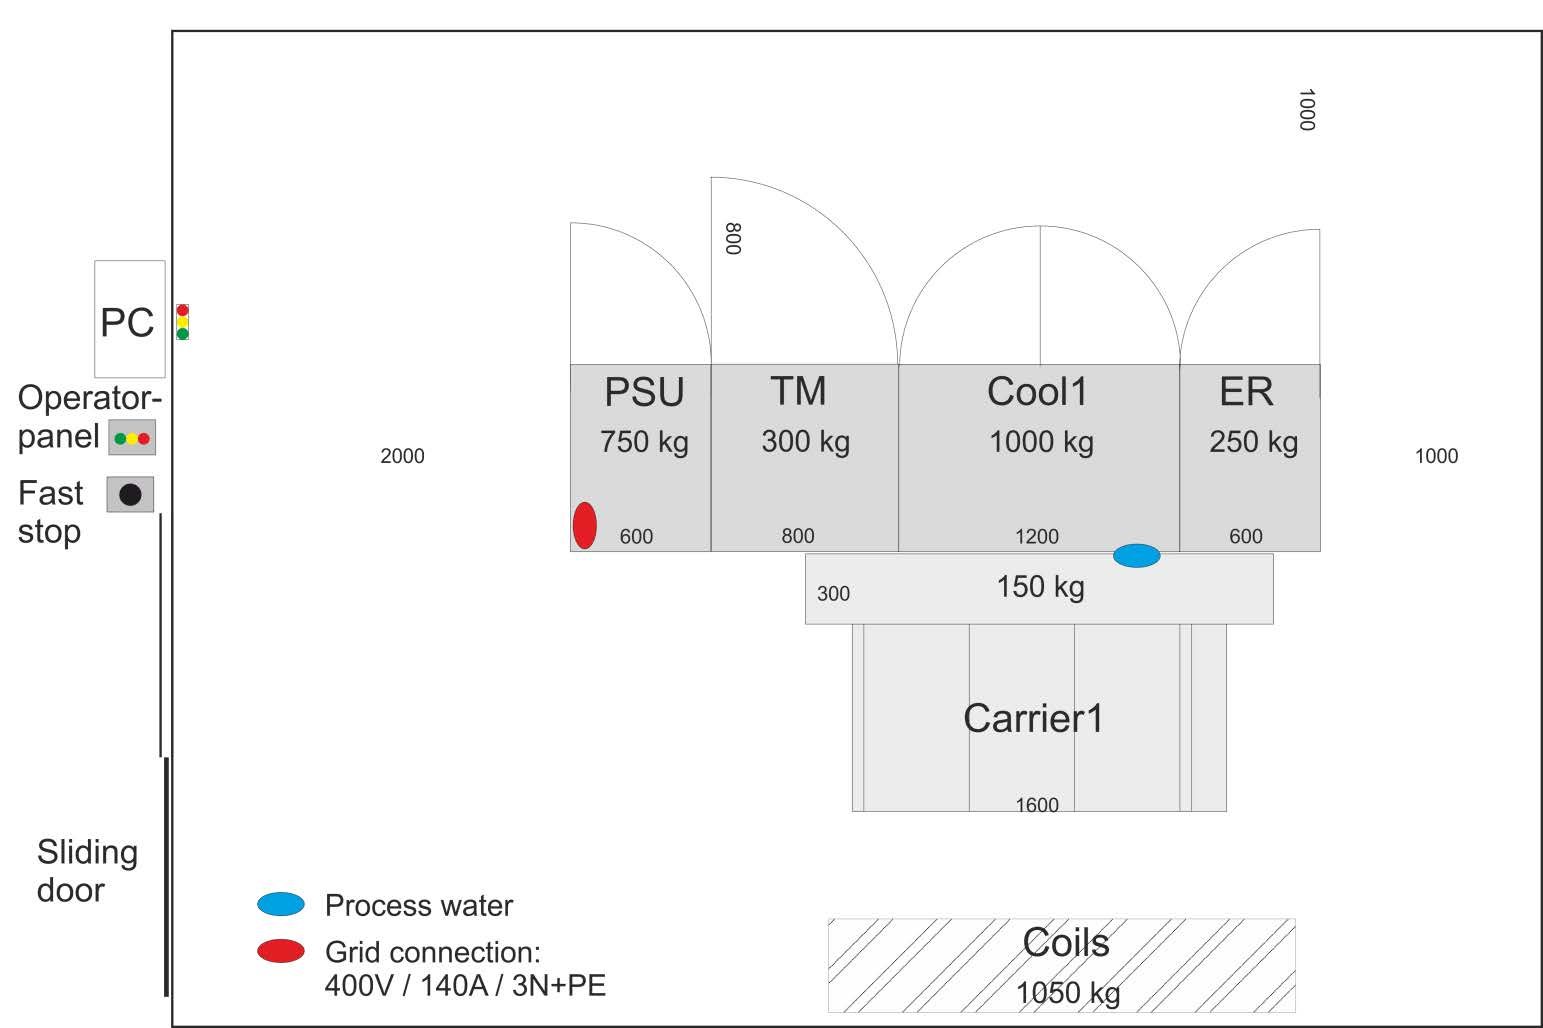
\includegraphics[width=0.8\textwidth]{Grafiken/Test Cabin.jpg}
    \caption{Aufbau des Teststandes}
    \label{fig:1. Aufbau des Teststandes}
    {Quelle: \cite*[7]{Main_Manuel_USTB2018}}
\end{figure}


%------------------------------------------------------------------------------------------------------
\subsubsection{Testmodule}
%------------------------------------------------------------------------------------------------------
Es gibt mehrere Testmodule, die auf dem Teststand laufen und verschieden Funktionen der Umrichter testen.
Einige der Funktionen eines DUT können mit dem gleichen Modus eines Testmoduls überprüft werden, indem die
entsprechenden Parameter ausgewählt werden.
Jeder Testablauf ist autonom und kann mehrmals ausgeführt werden, auch mit unterschiedlichen Parameter.
\\
Im Folgenden wird eine kurze Beschreibung der Funktionen der für diese Arbeit relevanten Testmoduls gegeben.

Driver Consumption Test:
Der Driver Consumption Test überprüft den Stromverbrauch des Treibers im Leerlauf und während Pulssprüngen.

Pulse Test:
Der Impulstest verfügt über drei Funktionsmodi.
\begin{itemize}
    \item Im Modus „Functional-Switching“ (FSW) kann überprüft werden, ob die Halbleiter generell schalten.
    \item Im Modus „Over-Current-Protection“ (OCP) kann die Überstromüberwachung weiche Kurzschlusse überprüft werden.
    Ein weicher Kurzschluss ist, wenn der Stromfluss nicht sofort und vollkommen unterbrochen wird.
    \item Im Modus „Dynamic-Short-Circuit-Protection“ (DSCP) wird das korrekte Verhalten der Treiberstufe in Bezug auf
    einen harten Kurzschluss, also ein vollständiger und sofortiger Kurzschluss, überprüft.
\end{itemize}

Power Test:
Mit diesem Test werden zwei verschiedene Funktionen getestet werden.
Der Burn-In-Test (BIT) dient dazu, die \ac{DUTs} zyklisch zu betreiben und so reale Betriebszustände zu simulieren.
Zudem kann mit Hilfe dieser Funktion die Kühltemperatur überprüft werden, um die korrekte Wärmeübertragung der Halbleiter zu überprüften.
\\
Während des Übertemperaturschutz-Tests (OTP) wird ein DUT ähnlich wie beim BIT nur mit reduzierter Kühlung betrieben, bis die maximal zulässige
Kühlkörpertemperatur erreicht ist und die Temperaturschutzschaltung auslöst.\cite*{Main_Manuel_USTB2018}
\color{red}     %Unfertig
%------------------------------------------------------------------------------------------------------
\subsubsection{Testablauf}
%------------------------------------------------------------------------------------------------------
Ein Test läuft wie folgt ab:

\begin{enumerate}
\item Die Umrichter werden auf dem Carrier befestigt, es werden meist 3 Umrichter gleichzeitig getastet, Abweichungen je nach Bauform der Umrichter.
Die Reihenfolge der elektrischen Phasen ist bei Draufsicht des Carriers von links nach rechts U-V-W.
\item Anschließen des Kühlkreislaufen, je nach Types Lüft- oder Wasserkühlung.
\item Die \ac{DUTs} werden mit den AC- und DC-Link-Kontakten verbinden.
\item Anbringen von Signalkabeln zwischen DUT und MerkurBox, so wie montieren von VCE-Klemmen an die AC-Kontakte der \ac{DUTs}.
\item
\item Durchführung des Driver Consumption Testes.
\item Durchführung des Pulse Testes.
\item Durchführung des Driver Power Testes.
\item Nach dem Durchlaufen eines Tests wird automatische ein XML-Datenfile mit den erhobenen Messdaten generiert, die enthalt die Messwerte und alle vorher bestimmten Einstellungen.
\end{enumerate}

